%%%%%%%%%%%%%%%%%%%%%%%%%%%%%%%%%%%%%%%%%%%%%%%%%%%%%%%%%%%%%%%%%%%%%%%%%%%%%%%
% Comparative Analysis of Quantum Finite Automata Models
%%%%%%%%%%%%%%%%%%%%%%%%%%%%%%%%%%%%%%%%%%%%%%%%%%%%%%%%%%%%%%%%%%%%%%%%%%%%%%%

\chapter{Comparative Analysis of Quantum Finite Automata Models}
\label{chap:comparative-analysis}

\section{Introduction}
This chapter provides a comprehensive comparison of quantum finite automata (QFA) models, structured into nine categories. We analyze their computational capabilities, language recognition properties, and practical trade-offs using schematic diagrams and tables. Key evaluation criteria include state complexity, error handling, and implementation feasibility. The models are organized as follows:
\begin{enumerate}
    \item One-Way QFAs
    \item One-and-a-Half-Way QFAs
    \item Two-Way QFAs
    \item Hybrid Classical-Quantum Models
    \item Generalised Models
    \item Specialised Models
    \item Promise Problem Solvers
    \item Interactive Models
    \item Abstract and Algebraic Models
\end{enumerate}
For each category, we summarize the operational mechanisms, present visual comparisons, and underline the most relevant models and their trade-offs. We then compare these groups across each other and conclude with an overall evaluation highlighting the most and least promising approaches.

%%%%%%%%%%%%%%%%%%%%%%%%%%%%%%%%%%%%%%%%%%%%%%%%%%%%%%%%%%%%%%%%%%%%%%%%%%%%%%%
\section{One-Way QFAs}
%%%%%%%%%%%%%%%%%%%%%%%%%%%%%%%%%%%%%%%%%%%%%%%%%%%%%%%%%%%%%%%%%%%%%%%%%%%%%%%

\subsection{Summary}
One-way QFAs process input left-to-right with varying measurement strategies:
\begin{itemize}
    \item \textbf{MO-1QFA}: Implements unitary evolution with a single final measurement. Recognizes reversible regular languages with zero error. State complexity is typically $O(\log n)$, but the model is non-closed under union.
    \item \textbf{MM-1QFA}: Uses intermediate measurements, enabling bounded-error recognition of all regular languages. It has an exponential state advantage over PFAs but suffers from measurement overhead.
    \item \textbf{LQFA}: Uses immediate post-symbol measurements to balance quantum coherence and decision making, particularly for parity languages.
    \item \textbf{1QFAC/CL-1QFA}: Hybrid models that combine classical state control with quantum updates, achieving efficient DFA simulation with constant quantum memory. (However, equivalence checking is undecidable \cite{hirvensalo2008}.)
    \item \textbf{A-QFA/MLQFA}: Enhanced models that use ancillary qubits (A-QFA) or multi-letter block processing (MLQFA) to recognize context-sensitive languages. MLQFA, however, suffer from exponential state growth in the block size $k$ \cite{ravikumar2003}.
\end{itemize}

\subsection{Schematic Diagram}
\begin{figure}[ht]
\centering
\begin{tikzpicture}[node distance=2.5cm, auto]
    \node[draw,rectangle,fill=blue!15,minimum width=2cm] (mo) {MO-1QFA};
    \node[draw,rectangle,fill=blue!15,minimum width=2cm, right=of mo] (mm) {MM-1QFA};
    \node[draw,rectangle,fill=blue!15,minimum width=2cm, below=of mo] (lq) {LQFA};
    \node[draw,rectangle,fill=blue!15,minimum width=2.8cm, right=of lq] (hybrid) {1QFAC/CL-1QFA};
    \node[draw,rectangle,fill=blue!15,minimum width=2.5cm, below=of lq] (enhanced) {A-QFA/MLQFA};
    
    \draw[->,thick] (mo) -- (mm) node[midway,above] {\small +Measurements};
    \draw[->,thick] (mo) -- (lq) node[midway,left] {\small +Collapse Risk};
    \draw[->,thick] (lq) -- (hybrid) node[midway,above] {\small +Classical Control};
    \draw[->,thick] (hybrid) -- (enhanced) node[midway,right] {\small +Ancillas/Blocks};
\end{tikzpicture}
\caption{Hierarchy of one-way QFAs (arrows indicate added features).}
\label{fig:one_way_hierarchy}
\end{figure}

\subsection{Tabular Comparison}
\begin{table}[ht]
\centering
\caption{Comparison of One-Way QFA Models}
\label{tab:one_way}
\begin{tabular}{|l|c|c|c|}
\hline
\textbf{Model} & \textbf{Language Class} & \textbf{State Complexity} & \textbf{Key Limitation} \\ \hline
MO-1QFA   & Reversible Regular & $O(\log n)$ & Non-closed under union \\ \hline
MM-1QFA   & Regular (bounded error) & $O(\log n)$ & Measurement overhead \\ \hline
1QFAC     & Regular & $O(1)$ (quantum) & Undecidable equivalence \\ \hline
MLQFA     & Context-sensitive & $O(2^k)$ & Exponential in $k$ \\ \hline
\end{tabular}
\end{table}

\subsection{Key Findings}
Hybrid models (1QFAC/CL-1QFA) provide an optimal balance between quantum efficiency and classical reliability. Although MLQFA extend language recognition capabilities, their exponential state growth limits practical applicability.

%%%%%%%%%%%%%%%%%%%%%%%%%%%%%%%%%%%%%%%%%%%%%%%%%%%%%%%%%%%%%%%%%%%%%%%%%%%%%%%
\section{One-and-a-Half-Way QFAs}
%%%%%%%%%%%%%%%%%%%%%%%%%%%%%%%%%%%%%%%%%%%%%%%%%%%%%%%%%%%%%%%%%%%%%%%%%%%%%%%

\subsection{Summary}
The 1.5-way QFA extends the one-way paradigm by permitting a limited lookback through a fixed-size sliding window. Key points include:
\begin{itemize}
    \item Processes nested languages (e.g., $\{ww^Rw\}$) in linear time.
    \item Outperforms pure one-way models in recognition power.
    \item Restricted by the fixed window size $k$, which limits handling of unbounded context.
\end{itemize}

\subsection{Schematic Diagram}
\begin{figure}[ht]
\centering
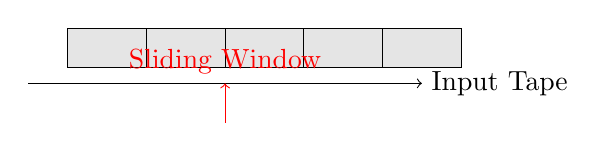
\begin{tikzpicture}
    \draw[->] (0,0) -- (5,0) node[right] {Input Tape};
    \foreach \x in {0.5,1.5,...,4.5} 
        \draw[fill=gray!20] (\x,0.2) rectangle (\x+1,0.7);
    \draw[red,->] (2.5,-0.5) -- (2.5,0) node[above] {Sliding Window};
\end{tikzpicture}
\caption{1.5-way QFA operation with a sliding window mechanism.}
\label{fig:1.5qfa}
\end{figure}

%%%%%%%%%%%%%%%%%%%%%%%%%%%%%%%%%%%%%%%%%%%%%%%%%%%%%%%%%%%%%%%%%%%%%%%%%%%%%%%
\section{Two-Way QFAs}
%%%%%%%%%%%%%%%%%%%%%%%%%%%%%%%%%%%%%%%%%%%%%%%%%%%%%%%%%%%%%%%%%%%%%%%%%%%%%%%

\subsection{Summary}
Two-way QFAs enable full bidirectional tape access, which allows them to recognize more complex (non-regular) languages:
\begin{itemize}
    \item \textbf{2QFA}: A pure quantum two-way model capable of recognizing languages such as $\{a^nb^n\}$.
    \item \textbf{2QCFA/kTQCFA}: Hybrid variants incorporating classical control, often achieving recognition (e.g., palindromes or $k$-tape dependencies) with reduced quantum memory.
\end{itemize}

\subsection{Schematic Diagram and Table}
\begin{figure}[ht]
\centering
\begin{tikzpicture}[node distance=2cm]
    \node[draw,circle,fill=red!20] (q1) {$q_1$};
    \node[draw,circle,fill=red!20,right=of q1] (q2) {$q_2$};
    \draw[<->,thick] (q1) -- node[midway, above] {Left/Right Moves} (q2);
\end{tikzpicture}
\caption{Bidirectional transitions in Two-Way QFAs.}
\label{fig:two_way}
\end{figure}

\begin{table}[ht]
\centering
\caption{Two-Way QFA Comparison}
\label{tab:two_way}
\begin{tabular}{|l|c|c|}
\hline
\textbf{Model} & \textbf{Quantum States} & \textbf{Expressiveness} \\ \hline
2QFA  & Linear in input & Non-regular languages \\ \hline
2QCFA & Constant & Context-sensitive languages \\ \hline
kTQCFA & $O(k)$ & $k$-tape dependencies \\ \hline
\end{tabular}
\end{table}

%%%%%%%%%%%%%%%%%%%%%%%%%%%%%%%%%%%%%%%%%%%%%%%%%%%%%%%%%%%%%%%%%%%%%%%%%%%%%%%
\section{Hybrid Classical-Quantum Models}
%%%%%%%%%%%%%%%%%%%%%%%%%%%%%%%%%%%%%%%%%%%%%%%%%%%%%%%%%%%%%%%%%%%%%%%%%%%%%%%

\subsection{Summary}
Hybrid models integrate classical logic with quantum processing:
\begin{itemize}
    \item \textbf{SQA}: Combines classical steering with quantum evolution.
    \item \textbf{QCPA}: Utilizes parity-based switching between classical and quantum modes.
    \item \textbf{BCQFA}: Employs blind counters to process balanced languages.
\end{itemize}

\subsection{Schematic Diagram}
\begin{figure}[ht]
\centering
\begin{tikzpicture}[node distance=2cm]
    \node[draw,rectangle,fill=green!20] (classical) {Classical Control};
    \node[draw,rectangle,fill=blue!20,right=of classical] (quantum) {Quantum Register};
    \draw[<->,thick] (classical) -- node[above] {Synchronization} (quantum);
\end{tikzpicture}
\caption{Architecture of a hybrid classical-quantum model.}
\label{fig:hybrid}
\end{figure}

\subsection{Comparative Insights}
Hybrid models (especially 1QFAC/CL-1QFA) provide a favorable balance of classical robustness and quantum speedup, making them among the most promising for practical implementations.

%%%%%%%%%%%%%%%%%%%%%%%%%%%%%%%%%%%%%%%%%%%%%%%%%%%%%%%%%%%%%%%%%%%%%%%%%%%%%%%
\section{Generalised Models}
%%%%%%%%%%%%%%%%%%%%%%%%%%%%%%%%%%%%%%%%%%%%%%%%%%%%%%%%%%%%%%%%%%%%%%%%%%%%%%%

\subsection{Summary}
Generalised QFAs extend the conventional unitary framework by incorporating non-unitary evolution:
\begin{itemize}
    \item \textbf{gQFA}: Uses \gls{cptp} maps to model noise \cite{gruska2005}.
    \item \textbf{MO-1GQFA/MM-1GQFA}: Generalised versions of one-way QFAs with enhanced robustness.
    \item \textbf{OTQFA}: Incorporates Lindbladian dynamics to explicitly handle decoherence.
\end{itemize}

\subsection{Tabular Comparison}
\begin{table}[ht]
\centering
\caption{Generalised QFA Characteristics}
\label{tab:general}
\begin{tabular}{|l|c|c|}
\hline
\textbf{Model} & \textbf{Decoherence Handling} & \textbf{Complexity} \\ \hline
gQFA   & CPTP maps (Markovian noise) & Quadratic slowdown \\ \hline
OTQFA & Lindbladian operators & PSPACE-level \\ \hline
\end{tabular}
\end{table}

\subsection{Comparative Insights}
While generalised models are crucial for addressing realistic noise, their increased complexity limits near-term practical deployment relative to simpler hybrid models.

%%%%%%%%%%%%%%%%%%%%%%%%%%%%%%%%%%%%%%%%%%%%%%%%%%%%%%%%%%%%%%%%%%%%%%%%%%%%%%%
\section{Specialized Models}
%%%%%%%%%%%%%%%%%%%%%%%%%%%%%%%%%%%%%%%%%%%%%%%%%%%%%%%%%%%%%%%%%%%%%%%%%%%%%%%

\subsection{Summary}
Specialized QFAs incorporate additional memory structures to extend their computational power:
\begin{itemize}
    \item \textbf{QQA/QPA}: Utilize quantum queues or stacks to recognize context-sensitive or EXPTIME languages.
    \item \textbf{PSQFA}: Leverage postselection to amplify correct outcomes under idealized conditions.
\end{itemize}

\subsection{Schematic Diagram}
\begin{figure}[ht]
\centering
\begin{tikzpicture}
    \node[draw,cylinder,fill=yellow!20,shape aspect=3] (queue) at (0,0) {Quantum Queue};
    \node[draw,rectangle,fill=blue!20,right=of queue] (control) {Control Unit};
    \draw[->] (control) -- (queue) node[midway,above] {Enqueue/Dequeue};
\end{tikzpicture}
\caption{Architecture of a quantum queue automaton.}
\label{fig:qqa}
\end{figure}

\subsection{Comparative Insights}
Although specialized models can recognize language classes beyond regular and context-free, their increased state complexity and error management issues make them less attractive for practical implementations.

%%%%%%%%%%%%%%%%%%%%%%%%%%%%%%%%%%%%%%%%%%%%%%%%%%%%%%%%%%%%%%%%%%%%%%%%%%%%%%%
\section{Promise Problem Solvers}
%%%%%%%%%%%%%%%%%%%%%%%%%%%%%%%%%%%%%%%%%%%%%%%%%%%%%%%%%%%%%%%%%%%%%%%%%%%%%%%

\subsection{Summary}
Promise problem solvers are tailored for inputs that meet specific conditions:
\begin{itemize}
    \item \textbf{Exact-QFA}: Achieves zero-error recognition for promise problems (e.g., EVENODD$_k$), but its applicability is limited.
    \item \textbf{BEQFA}: Allows bounded error recognition, broadening the range of recognizable languages while tolerating implementation inaccuracies.
\end{itemize}

\subsection{Tabular Comparison}
\begin{table}[ht]
\centering
\caption{Promise Problem Solvers: Characteristics}
\label{tab:promise}
\begin{tabular}{|l|c|c|c|}
\hline
\textbf{Model} & \textbf{Error Guarantee} & \textbf{Applicability} & \textbf{Complexity} \\ \hline
Exact-QFA & Zero error (for promises) & Narrow domain & Moderate \\ \hline
BEQFA    & Bounded error & Broader classes & Low to moderate \\ \hline
\end{tabular}
\end{table}

\subsection{Comparative Insights}
Promise problem solvers deliver high reliability under specific input conditions but are less flexible in general-purpose language recognition.

%%%%%%%%%%%%%%%%%%%%%%%%%%%%%%%%%%%%%%%%%%%%%%%%%%%%%%%%%%%%%%%%%%%%%%%%%%%%%%%
\section{Interactive Models}
%%%%%%%%%%%%%%%%%%%%%%%%%%%%%%%%%%%%%%%%%%%%%%%%%%%%%%%%%%%%%%%%%%%%%%%%%%%%%%%

\subsection{Summary}
Interactive models extend QFA capabilities via communication protocols between a prover and a verifier:
\begin{itemize}
    \item \textbf{QIP(1QFA)}: Single-prover interactive systems for regular languages, operating with $O(\log n)$ qubits \cite{yakaryilmaz2013verification}.
    \item \textbf{QMIP(2QCFA)}: Multi-prover systems utilizing entanglement to recognize even recursively enumerable languages, albeit with high resource demands.
\end{itemize}

\subsection{Schematic Diagram and Table}
\begin{figure}[ht]
\centering
\begin{tikzpicture}[node distance=2cm, auto]
    \node[draw, ellipse, fill=purple!10] (Prover) {Prover};
    \node[draw, ellipse, fill=purple!10, right=of Prover, node distance=4cm] (Verifier) {Verifier (QFA)};
    \draw[<->, thick] (Prover) -- node[midway, above] {Interaction} (Verifier);
\end{tikzpicture}
\caption{Interactive protocol between prover and verifier in QIP systems.}
\label{fig:interactive}
\end{figure}

\begin{table}[ht]
\centering
\caption{Interactive Model Comparison}
\label{tab:interactive}
\begin{tabular}{|l|c|c|}
\hline
\textbf{Model} & \textbf{Provers} & \textbf{Practicality} \\ \hline
QIP(1QFA) & 1 & Moderate \\ \hline
QMIP(2QCFA) & Multiple & Experimental \\ \hline
\end{tabular}
\end{table}

\subsection{Comparative Insights}
Interactive models offer significant theoretical power and bridge automata with complexity theory. However, their high resource and network demands currently hinder practical deployment.

%%%%%%%%%%%%%%%%%%%%%%%%%%%%%%%%%%%%%%%%%%%%%%%%%%%%%%%%%%%%%%%%%%%%%%%%%%%%%%%
\section{Abstract and Algebraic Models}
%%%%%%%%%%%%%%%%%%%%%%%%%%%%%%%%%%%%%%%%%%%%%%%%%%%%%%%%%%%%%%%%%%%%%%%%%%%%%%%

\subsection{Summary}
Abstract models provide a high-level, algebraic perspective on QFA:
\begin{itemize}
    \item \textbf{abstract-QFA}: A unified algebraic framework expressing BQP languages, primarily theoretical \cite{manin1980computable}.
    \item \textbf{OLVA}: Models quantum logic using orthomodular lattices for niche applications.
    \item \textbf{MPSQFA}: Uses tensor network (matrix product state) methods to simulate quantum state evolution \cite{vidal2003efficient}.
\end{itemize}

\subsection{Tabular Comparison}
\begin{table}[ht]
\centering
\caption{Abstract Models: Characteristics}
\label{tab:abstract}
\begin{tabular}{|l|c|c|c|}
\hline
\textbf{Model} & \textbf{Theoretical Focus} & \textbf{Applicability} & \textbf{Complexity} \\ \hline
abstract-QFA & Algebraic formulation & Unification of QFA theory & High \\ \hline
OLVA        & Quantum logic framework & Niche applications & Very high \\ \hline
MPSQFA      & Tensor network simulation & Theoretical exploration & High \\ \hline
\end{tabular}
\end{table}

\subsection{Comparative Insights}
Abstract models are essential for advancing a unified theoretical foundation of quantum automata. Their high complexity and abstract nature, however, limit their immediate practical application.

%%%%%%%%%%%%%%%%%%%%%%%%%%%%%%%%%%%%%%%%%%%%%%%%%%%%%%%%%%%%%%%%%%%%%%%%%%%%%%%
\section{Overall Comparative Discussion and Final Evaluation}
%%%%%%%%%%%%%%%%%%%%%%%%%%%%%%%%%%%%%%%%%%%%%%%%%%%%%%%%%%%%%%%%%%%%%%%%%%%%%%%

\subsection{Cross-Category Comparisons}
The following trends emerge from our analysis:
\begin{itemize}
    \item \textbf{Expressiveness vs. Complexity:} One-way models are simple and resource-efficient but limited in expressive power. Two-way and interactive models offer higher expressiveness at the cost of increased control complexity and resource demands.
    \item \textbf{Hybrid Approaches:} Hybrid models (e.g., 1QFAC/CL-1QFA) efficiently bridge classical reliability with quantum speedup and are among the most promising for near-term applications (e.g., 1QFAC \cite{qiu2009}).
    \item \textbf{Generalised and Abstract Models:} While these approaches can handle realistic noise and unify theory, their complexity makes them less practical in the short term.
\end{itemize}

\subsection{Key Models and Promising Directions}
\begin{itemize}
    \item \textbf{Most Expressive (Theoretically):} QMIP(2QCFA) and abstract-QFA demonstrate extraordinary theoretical power but are experimentally challenging.
    \item \textbf{Most Practical:} MM-1QFA and hybrid models like 1QFAC offer a good balance between error control and state complexity.
    \item \textbf{Balanced Design:} 2QCFA, with constant quantum memory and polynomial time operation, represent a promising middle ground.
\end{itemize}

\subsection{Final Evaluation}
In summary, while theoretical models such as interactive and abstract QFAs push the boundaries of what quantum automata can achieve, hybrid and generalised models offer the most viable path toward practical quantum advantage in language recognition. Future research should focus on:
\begin{itemize}
    \item Developing robust error correction and state minimization techniques for hybrid architectures.
    \item Implementing hardware prototypes for 1.5-way and two-way models.
    \item Advancing algebraic frameworks to unify generalized and abstract models.
\end{itemize}

%%%%%%%%%%%%%%%%%%%%%%%%%%%%%%%%%%%%%%%%%%%%%%%%%%%%%%%%%%%%%%%%%%%%%%%%%%%%%%%
\section{Conclusion and Future Directions}
This chapter has presented a detailed comparative analysis of QFA models across nine categories. Key findings include:
\begin{itemize}
    \item \textbf{One-Way Models} are resource-efficient but limited in expressiveness.
    \item \textbf{1.5-Way and Two-Way Models} enhance recognition capabilities at the expense of increased complexity.
    \item \textbf{Hybrid Models} (e.g., 1QFAC/CL-1QFA) offer the best balance for practical applications.
    \item \textbf{Generalised Models} effectively handle realistic noise, though with higher complexity (e.g., Gruska's noise models \cite{gruska2005}).
    \item \textbf{Specialized Models} extend language recognition capabilities but are hampered by high state complexity and error management challenges.
    \item \textbf{Promise Problem Solvers} provide high reliability under strict input conditions, yet their applicability is narrow.
    \item \textbf{Interactive Models} push computational boundaries but require substantial resources.
    \item \textbf{Abstract and Algebraic Models} are crucial for theoretical unification, yet are currently less practical.
\end{itemize}
Overall, hybrid and generalised models emerge as the most promising for near-term quantum computing applications, while promise problem solvers, specialized, interactive, and abstract models continue to provide valuable insights for advancing the theoretical foundations of quantum automata.
